% quadrature.tex

\chapter{Quadrature numérique sur le Cubed-Sphere}


\section{Pré-requis} %% ***************************************************************************************

Si $f$ est une conction de $\mathcal{C}^{\infty}([a,b])$ alors la formule d'Euler MacLaurin s'écrit :

\begin{equation}
\dfrac{1}{b-a} \gint_a^b f(x)dx = \dfrac{f(a)+f(b)}{2} - \gsum_{j=1}^k (b-a)^{2j-1} \dfrac{b_{2j}}{(2j)!} \left( f^{(2j-1)}(b) - f^{(2j-1)}(a) \right) - \mathcal{O}\left( (b-a)^{(2k+2)} \right)
\label{eq:euler maclaurin}
\end{equation}

avec $b_{2j}$ les nombres de Bernoulli ($b_2=1/6$, $b_4=1/30$, ...).

Si on souhaite calculer $\gint_{-\pi/4}^{\pi/4} f(\xi,\eta)d\xi$ en utilisant la formule d'Euler MacLaurin \eqref{eq:euler maclaurin} sur les sous intervalles $[\xi_i, \xi_{i+1}]$ (formule d'Euler MacLaurin composite) avec $\xi_i= i \times \Delta \xi$, $\Delta \xi = \dfrac{\pi}{2(N+1)}$ on obtient :

\begin{equation}
\begin{array}{rl}
\gint_{-\pi/4}^{\pi/4} f(\xi,\eta)d\xi & = \dfrac{\Delta \xi}{2} f(\xi_{-\frac{N}{2}},\eta) +  \Delta \xi \gsum_{i=-\frac{N}{2}+1}^{\frac{N}{2}-1} f(\xi_i,\eta) + \frac{\Delta \xi}{2} f(\xi_{\frac{N}{2}},\eta)- ...\\
                                       & ... - \dfrac{b_2}{2!} \Delta \xi^2 \left( \partial_\xi f(\xi_{\frac{N}{2}},\eta) - \partial_\xi f(\xi_{-\frac{N}{2}},\eta) \right) + \mathcal{O} \left( \Delta \xi ^4 \right)
\end{array}
\end{equation}

On pose : $$I = \left\lbrace i\in\mathbb{N} \text{ tels que } -\frac{N}{2}+1 \leq i \leq \frac{N}{2}-1 \right\rbrace$$ et on applique la même méthode dans la direction de $\eta$  :

\begin{equation}
\begin{array}{rl}
\gint_{-\pi/4}^{\pi/4} \gint_{-\pi/4}^{\pi/4} f(\xi,\eta)d\xi d\eta &  = \Delta \xi \Delta \eta \gsum_{i \in I} \gsum_{j \in I} f_{i,j} + ... \\

 & ... + \dfrac{\Delta \xi \Delta \eta}{2} \left[ \gsum_{i \in I} \left(  f_{i,\frac{N}{2}} + f_{i,-\frac{N}{2}})  \right) + \gsum_{j \in I} \left(  f_{\frac{N}{2},j} + f_{-\frac{N}{2},j}  \right) \right] - ... \\
 
 & ... + \dfrac{\Delta \xi \Delta \eta}{4} \left[ f_{\frac{N}{2},\frac{N}{2}}+f_{-\frac{N}{2},\frac{N}{2}}+f_{\frac{N}{2},-\frac{N}{2}}+f_{-\frac{N}{2},-\frac{N}{2}} \right] + ... \\
 
 &  ... - \dfrac{b_2}{2!} \Delta \xi \Delta \eta \left[ \Delta \eta \gsum_{i \in I} \left(  \partial_{\eta }f_{i,\frac{N}{2}} -  \partial_{\eta }f_{i,-\frac{N}{2}}  \right) + \Delta \xi \gsum_{j \in I} \left(   \partial_{\xi }f_{\frac{N}{2},j} - \partial_{\xi }f_{-\frac{N}{2},j}  \right) \right] + ... \\

  & ... - b_2 \dfrac{\Delta \xi \Delta \eta^2}{4} \left[ \partial_{\eta} f_{-\frac{N}{2},\frac{N}{2}} - \partial_{\eta} f_{-\frac{N}{2},-\frac{N}{2}} + \partial_{\eta} f_{\frac{N}{2},\frac{N}{2}} -\partial_{\eta} f_{\frac{N}{2},-\frac{N}{2}}  \right] - ... \\
 
  & ... - b_2 \dfrac{\Delta \xi^2 \Delta \eta}{4} \left[ \partial_{\xi} f_{\frac{N}{2},\frac{N}{2}} + \partial_{\xi} f_{\frac{N}{2},-\frac{N}{2}} - \partial_{\xi} f_{-\frac{N}{2},\frac{N}{2}} -\partial_{\xi} f_{-\frac{N}{2},-\frac{N}{2}}  \right] + ... \\
  
  & ... + \mathcal{O} \left( \Delta \xi^4, \Delta \eta^4 \right)
  \end{array}
\label{eq:euler maclaurin 2d composite}
\end{equation}

avec l'abus de notation $f_{i,j} = f(\xi_i, \eta_j)$ pour tous $i$ et $j$.

On note l'intégrale sur le panel $(K)$ (avec $K \in \left\lbrace I, II, III, IV, V, VI \right\rbrace$) de $h$ :
$$I^{(K)}(h) = \gint_{(K)} h(\mathbf{x}) d \sigma (\mathbf{x}).$$

Après changement de variable $\psi^{(K)} : (\xi, \eta) \in [-\pi/4, \pi/4]^2 \mapsto \mathbf{x} \in \mathbb{S}_a^2$, on obtient :

\begin{equation}
\begin{array}{rcl}
I^{(K)}(h) & = &  \gint_{\psi^{(K)^{-1}}\left((K)\right)}  h\left( \psi^{(K)^{-1}}\right) |Jac ( \psi^{(K)} )|d\xi d\eta \\
& = & \gint_{-\pi/4}^{\pi/4}\gint_{-\pi/4}^{\pi/4} h(\xi, \eta) \sqrt{\mathbf{\bar{G}}^{(K)}(\xi, \eta)} d \xi d \eta.
\end{array}
\end{equation}

La formule d'Euler MacLaurin \eqref{eq:euler maclaurin 2d composite} peut être appliquée sur chaque panel de la Cubed-Sphère en posant $f(\xi,\eta)=h(\xi,\eta)\sqrt{\mathbf{\bar{G}}^{(K)}(\xi, \eta)}$. On dispose alors d'une intègrale sur la sphère complète :

\begin{equation}
I(h)=\gint_{\mathbb{S}_a^2} h(\mathbf{x})d\sigma(\mathbf{x}) = \gsum_{K = I}^{VI} I^{(K)}(h)
\end{equation}














\section{Généralités}

Dans cette partie, on s'intéresse à des formules de quadrature numérique de la forme :

\begin{equation}
Q^{(K)}(h)= \gsum_{j=-N/2}^{N/2} \Delta \xi \Delta \eta \gsum_{i=-N/2}^{N/2} \omega_{i,j} h(\xi_i,\eta_j) \sqrt{\overline{\mathbf{G}}(\xi_i,\eta_j)}
\label{eq: quadrature generale}
\end{equation}

avec $(\omega_{i,j})_{i,j}$ des réels positifs vérifiant la propriété suivante :

\begin{equation}
\omega_{i,j}=\omega_{-i,j}=\omega_{i,-j}=\omega_{-i,-j} \hspace{0.8cm} \text{ pour tous } i \text{ et } j
\label{hyp: prop triangulaire}
\end{equation}

Un produit scalaire hermitien est issu de la formule de quadrature précédente. $\mathbf{u}$ et $\mathbf{v}$ sont deux données sur la Cubed-Sphere : pour tous $K \in \lbrace I, ..., VI \rbrace$, $-\frac{N}{2} \leq i,j \leq \frac{N}{2}$ alors $\mathbf{u}_{i,j}^{(K)} \in \mathbb{C}$ et $\mathbf{v}_{i,j}^{(K)} \in \mathbb{C}$. Le produit scalaire hermitien, noté $< \cdot, \cdot >_{CS}$, est donné par :

\begin{equation}
<\mathbf{u}, \mathbf{v}>_{CS} = \Delta \xi \Delta \eta \gsum_{K=I}^{VI} \gsum_{i=-\frac{N}{2}}^{\frac{N}{2}} \gsum_{i=-\frac{N}{2}}^{\frac{N}{2}} \omega_{i,j} \sqrt{\overline{\mathbf{G}_{i,j}}} \mathbf{u}_{i,j}^{(K)} \bar{\mathbf{v}}_{i,j}^{(K)}
\end{equation}

\begin{proposition}
$< \cdot, \cdot >_{CS}$ définit un produit scalaire hermitien sur la sphère.
\end{proposition}

\begin{proof}
\begin{itemize}
\item pour tout $\mathbf{x}$ donné sur la Cubed-Sphere, la forme : $<\cdot, \mathbf{x}>_{CS}$ est linéaire et $<\mathbf{x}, \cdot>_{CS}$ est semilinéaire. Ainsi $<\cdot, \cdot>_{CS}$ est sesquilinéaire.

\item Pour tous $\mathbf{x}$ et $\mathbf{y}$ donnés sur la Cubed-Sphere, alors :
\begin{equation*}
\begin{array}{rcl}
< \mathbf{x} , \mathbf{y} >_{CS} & = & \Delta \xi \Delta \eta \gsum_{K=I}^{VI} \gsum_{i=-\frac{N}{2}}^{\frac{N}{2}} \gsum_{i=-\frac{N}{2}}^{\frac{N}{2}} \omega_{i,j} \sqrt{\overline{\mathbf{G}}_{i,j}} \mathbf{x}_{i,j}^{(K)} \bar{\mathbf{y}}_{i,j}^{(K)} \\

& $=$ & \overline{<\mathbf{y}, \mathbf{x}>_{CS}}
\end{array}
\end{equation*}
donc $<\cdot,\cdot>_{CS}$ est hermitienne,
\item Soit $\mathbf{x}$ donné sur la Cubed-Sphere, si $<\mathbf{x},\mathbf{x}>=0$ alors pour tous $i$, $j$ et $K$, on a : $\mathbf{x}_{i,j}^{(K)}\bar{\mathbf{x}}_{i,j}^{(K)} = 0$ car les coefficients de linéarité  $\Delta \xi \Delta \eta \omega_{i,j} \sqrt{\overline{\mathbf{G}}_{i,j}}$ sont tous positif et non nuls. D'où $\mathbf{x} = 0$. Et $<\cdot, \cdot >_{CS}$ est définie positive.
\end{itemize}
\end{proof}


Le théorème suivant est alors vérifié :

\begin{theoreme}
Soient deux harmoniques sphériques restreintes à la sphère $\mathbf{Y}_m^l$ et $\mathbf{Y}_{m'}^{l'}$ avec $m, m' \in \mathbb{N}$, $|l| \leq m$ et $|l'| \leq m'$ alors :
\begin{equation}
<\mathbf{Y}_{m}^{l},\mathbf{Y}_{m'}^{l'}> = 0 
\end{equation}
si $m+m'$ ou $l+l'$ est impair.
\end{theoreme}

\begin{proof}
Notons $Y_m^l$ une harmonique sphèrique et $\mathbf{Y}_m^l$ sa restriction au maillage Cubed-Sphère.
Commençons par remarque que si $(\lambda, \theta)$ représente les coordonnées latitude-longitude d'un point de la sphère :
\begin{itemize}
\item $Y_m^l (\lambda, \theta) = (-1)^{m+l} Y_m^l (\lambda, - \theta)$, 
\item $Y_m^l(\lambda, \theta) = (-1)^p Y_m^l \left( \lambda + p \frac{\pi}{m}, \theta \right)$,
\item $Y_m^l(\lambda,\theta)=\overline{Y}_m^l(-\lambda,\theta)$.
\end{itemize}

Dans la suite de cette démonstration, nous noterons :

$$
S_(K) = \Delta \xi \Delta \eta \gsum_{i = \frac{N}{2}}^{\frac{N}{2}} \gsum_{j = \frac{N}{2}}^{\frac{N}{2}} \omega_{i,j} \sqrt{\overline{\mathbf{G}}_{i,j}} \left(\mathbf{Y}_m^l\right)_{i,j}^{(K)} \left(\bar{\mathbf{Y}}_{m'}^{l'}\right)_{i,j}^{(K)}
$$

Donc :

$$
S=<\mathbf{Y}_m^l,\mathbf{Y}_{m'}^{l'}>_{CS} = \gsum_{K=I}^{VI} S_{(K)}
$$

En utilisant les symétries évoquées ci dessous, on montre que :

\begin{equation*}
\begin{array}{rcl}
S_I & = & \Delta \xi \Delta \eta \gsum_{i = \frac{N}{2}}^{\frac{N}{2}} \gsum_{j = \frac{N}{2}}^{\frac{N}{2}} \omega_{i,j} \sqrt{\overline{\mathbf{G}}_{i,j}} \left(\mathbf{Y}_m^l\right)_{i,j}^{(I)} \left(\bar{\mathbf{Y}}_{m'}^{l'}\right)_{i,j}^{(I)} \\
& = & (-1)^{l+l'} \Delta \xi \Delta \eta \gsum_{i = \frac{N}{2}}^{\frac{N}{2}} \gsum_{j = \frac{N}{2}}^{\frac{N}{2}} \omega_{i,j} \sqrt{\overline{\mathbf{G}}_{i,j}} \left(\mathbf{Y}_m^l\right)_{i,j}^{(III)} \left(\bar{\mathbf{Y}}_{m'}^{l'}\right)_{i,j}^{(III)} \\
& = & (-1)^{l+l'} S_{III}
\end{array}
\end{equation*}

De même :

\begin{itemize}
\item $S_{II} = (-1)^{l+l'} S_{IV}$,
\item $S_{I} = (-1)^{l+l'} S_{III}$,
\end{itemize}

et en utilisant la symétrie passant du panel V au panel VI, on a $S_{V} = (-1)^{m+m'+l+l'}S_{VI}$.

De ces égalités, on peut déduire que :

\begin{equation}
S=(1+(-1)^{l+l'})(S_I+S_II)+(1+(-1)^{l+l'+m+m'})S_V
\end{equation}

Les points du panel $I$ se retrouvent par rotation d'un angle de $\frac{\pi}{2}$, or : $Y_m^l\left(\lambda + \frac{\pi}{2}, \theta \right) = \exp \left[ - i l \dfrac{\pi}{2} \right] Y_m^l(\lambda, \theta)$.

Dès lors :

$$
S_{II} = \exp \left[ - i (l+l') \dfrac{\pi}{2} \right] S_I
$$

d'où :

\begin{equation}
S=\left(1+(-1)^{l+l'}\right)\left( \exp \left[ - i (l+l') \dfrac{\pi}{2} \right] +1 \right) S_I + (1+(-1)^{l+l'+m+m'})S_V
\label{eq:pdt scal nul 1}
\end{equation}

$S=0$ si $m+m'$ et $l+l'$ sont impairs tous les deux.
Le problème est à présent de savoir quand $S_I$ et $S_V$ s'annulent. 

Pour $S_I$, on souhaite utiliser les symétries selon $(Oz)$ et $(Oy)$. On nomme $S_i$ avec $i$ entre 1 et 4 la partie de la somme $S_I$ contenant les points associés aux zones suivantes (voir Figure \ref{fig: zones panel I}) :

\begin{itemize}
\item $1$: les points $(x,y,z)$ du panel I tels que $y<0$ et $z>0$,
\item $2$: les points $(x,y,z)$ du panel I tels que $y<0$ et $z<0$,
\item $3$: les points $(x,y,z)$ du panel I tels que $y>0$ et $z<0$,
\item $4$: les points $(x,y,z)$ du panel I tels que $y>0$ et $z>0$.
\end{itemize}

\begin{figure}
\begin{center}
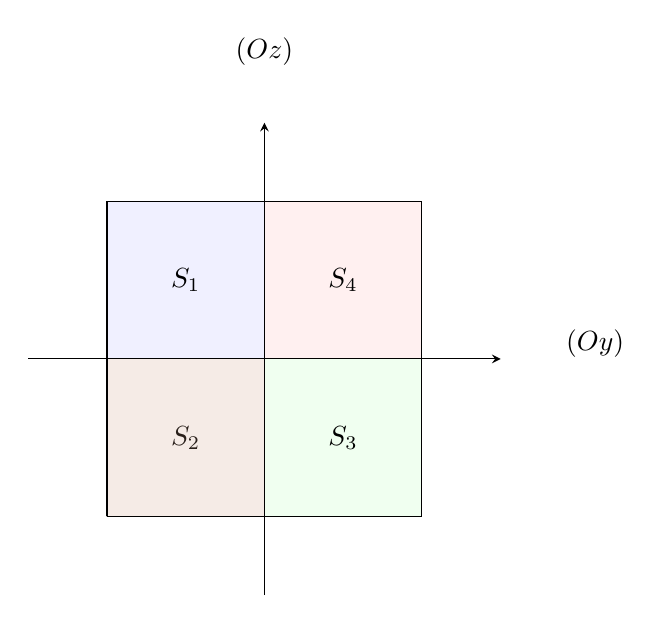
\begin{tikzpicture}[scale=2]
\filldraw[draw=black,fill=blue!30!white,opacity=0.20]
	plot (-1,0)
	-- plot (-1,1)
	-- plot (0,1)
	-- plot (0,0)
	-- cycle;	
\draw (-0.5,0.5) node{$S_1$} ;

\filldraw[draw=black,fill=red!30!white,opacity=0.20]
	plot (0,0)
	-- plot (0,1)
	-- plot (1,1)
	-- plot (1,0)
	-- cycle;	
\draw (-0.5,-0.5) node{$S_2$} ;

\filldraw[draw=black,fill=green!30!white,opacity=0.20]
	plot (0,0)
	-- plot (1,0)
	-- plot (1,-1)
	-- plot (0,-1)
	-- cycle;	
\draw (0.5,-0.5) node{$S_3$} ;

\filldraw[draw=black,fill=Sepia!30!white,opacity=0.20]
	plot (0,0)
	-- plot (0,-1)
	-- plot (-1,-1)
	-- plot (-1,0)
	-- cycle;	
\draw (0.5,0.5) node{$S_4$} ;

\draw (-1,-1) -- (1,-1) ;
\draw (-1,1) -- (1,1) ;
\draw (1,1) -- (1,-1) ;
\draw (-1,1) -- (-1,-1) ;
\draw [>=stealth, ->](-1.5,0) -- (1.5,0) ;
\draw (2.1,0.25) node[below]{$(Oy)$} ;
\draw [>=stealth, ->](0,-1.5) -- (0,1.5) ;
\draw (0,2.1) node[below]{$(Oz)$} ;
\end{tikzpicture}
\end{center}
\caption{Représentation schématique des zones $S_1$ à $S_4$ sur le panel I}
\label{fig: zones panel I}
\end{figure}

En tenant compte des symétries autour de $(Oz)$ et $(Oy)$, il est aisé de voir que :

\begin{equation*}
\begin{array}{rcl}
S_I & = & S_1 + S_2 + S_3 + S_4 \\
    & = & S_1 + S_2 + \bar{S}_1 + \bar{S}_2 \\
    & = & (1+(-1)^{l+l'+m+m'})(S_1+\bar{S}_1)
\end{array}
\end{equation*}

Ainsi $S_I=0$ si $l+l'$ pair et $m+m'$ impair, d'où $S=0$ en tenant compte de \eqref{eq:pdt scal nul 1}.

En ce qui concerne $S_V$, on nomme $S_a$ et $S_b$ les parties de la somme $S_V$ contenant les points associés aux zones suivantes (voir Figure \ref{fig: zones panel V}) :

\begin{itemize}
\item $a$: les points $(x,y,z)$ du panel V tels que $y<0$,
\item $b$: les points $(x,y,z)$ du panel V tels que $y>0$.
\end{itemize}


\begin{figure}
\begin{center}
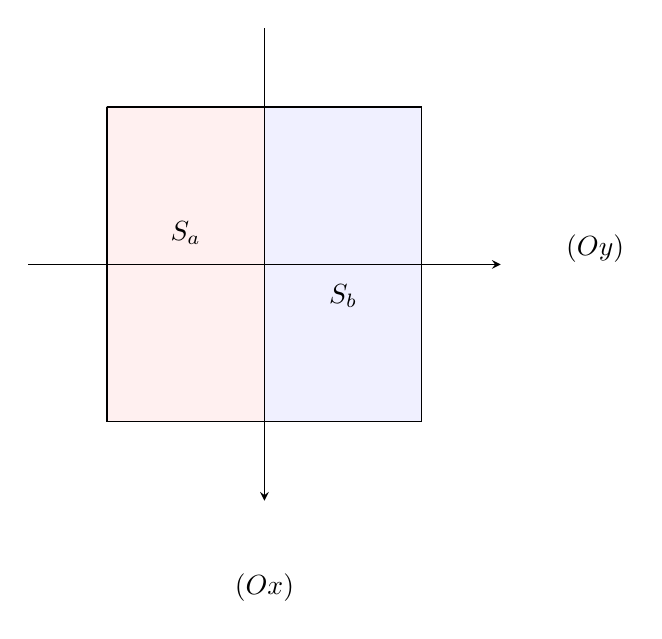
\begin{tikzpicture}[scale=2]
\filldraw[draw=black,fill=red!30!white,opacity=0.20]
	plot (-1,-1)
	-- plot (-1,1)
	-- plot (0,1)
	-- plot (0,-1)
	-- cycle;	
\filldraw[draw=black,fill=blue!30!white,opacity=0.20]
	plot (0,1)
	-- plot (1,1)
	-- plot (1,-1)
	-- plot (0,-1)
	-- cycle;	

\draw (-1,-1) -- (1,-1) ;
\draw (-1,1) -- (1,1) ;
\draw (1,1) -- (1,-1) ;
\draw (-1,1) -- (-1,-1) ;

\draw [>=stealth, ->](-1.5,0) -- (1.5,0) ;
\draw (2.1,0.25) node[below]{$(Oy)$} ;

\draw [>=stealth, ->](0,1.5) -- (0,-1.5) ;
\draw (0,-1.9) node[below]{$(Ox)$} ;

\draw (-0.5,0.2) node{$S_a$} ;
\draw (0.5,-0.2) node{$S_b$} ;

\end{tikzpicture}
\end{center}
\caption{Représentation schématique des zones $S_a$ et $S_b$ sur le panel V}
\label{fig: zones panel V}
\end{figure}

Alors $S_V=(1+(-1)^{l-l'})S_a$. $S_V=0$ si $l+l'$ est impair. Dans ce cas, $S=0$ et le résultat du théorème est prouvé.

 







\end{proof}


















\section{Quadrature de type Trapèzes}  %% ***************************************************************************************

On utilise une formule de quadrature $Q_{tpz}(h)$ visant à approcher $I^{(K)}(h)$ en utilisant la formule des trapèzes composites :

\begin{equation}
\gint_{a}^b f(x)dx \approx \dfrac{b-a}{N} \left[ \dfrac{f(a)+f(b)}{2} + \gsum_{k=1}^{N-1} f\left( a+k \dfrac{b-a}{N} \right) \right]
\label{eq:trapezes composites}
\end{equation}

Il s'agit en fait de l'intégration de l'interpolation de $f$ par une fonction affine par morceaux. On note immédiatement que la formule des trapèzes est exacte par construction pour $f$ affine.

En appliquant \eqref{eq:trapezes composites} sur un carré, on obtient :

\begin{equation}
\begin{split}
\gint_{-\pi/4}^{\pi/4} \gint_{-\pi/4}^{\pi/4} f(\xi,\eta)d\xi d\eta \approx \Delta \xi \Delta \eta \gsum_{i \in I} \gsum_{j \in I} f_{i,j} +  \dfrac{\Delta \xi \Delta \eta}{2} \left[ \gsum_{i \in I} \left(  f_{i,\frac{N}{2}} + f_{i,-\frac{N}{2}}  \right) + \gsum_{j \in I} \left(  f_{\frac{N}{2},j} + f_{-\frac{N}{2},j}  \right) \right] + ... \\
...+ \dfrac{\Delta \xi \Delta \eta}{4} \left[ f_{\frac{N}{2},\frac{N}{2}}+f_{-\frac{N}{2},\frac{N}{2}}+f_{\frac{N}{2},-\frac{N}{2}}+f_{-\frac{N}{2},-\frac{N}{2}} \right]- b_2 \dfrac{\Delta \xi \Delta \eta^2}{4} \left[ \partial_{\eta} f_{-\frac{N}{2},\frac{N}{2}} - \partial_{\eta} f_{-\frac{N}{2},-\frac{N}{2}} \right]
\end{split}
\label{eq:trapezes 2d composite}
\end{equation}

La formule de quadrature sur le panel $(K)$ est alors la suivante :

\begin{equation}
Q_{tpz}^{(K)}(h)=\gsum_{i = -\frac{N}{2}}^{\frac{N}{2}}\gsum_{j = -\frac{N}{2}}^{\frac{N}{2}} \Delta \xi \Delta \eta \omega_{i,j} h(\xi_i, \eta_j) \sqrt{\mathbf{\bar{G}}^{(K)}(\xi_i, \eta_j)}
\label{eq:trapezes par panel}
\end{equation}

avec :

\begin{itemize}
\item $\omega_{-\frac{N}{2},-\frac{N}{2}}=\omega_{\frac{N}{2},-\frac{N}{2}}=\omega_{-\frac{N}{2},\frac{N}{2}}=\omega_{\frac{N}{2},\frac{N}{2}}=\frac{1}{4}$,
\item $\omega_{i,\frac{N}{2}}=\omega_{i,-\frac{N}{2}}=\frac{1}{2}$ pour $-\frac{N}{2}+1 \leq i \leq \frac{N}{2}-1$,
\item $\omega_{\frac{N}{2},j}=\omega_{-\frac{N}{2},j}=\frac{1}{2}$ pour $-\frac{N}{2}+1 \leq j \leq \frac{N}{2}-1$,
\item $\omega_{i,j}=1$ dans tous les autres cas.
\end{itemize}

\begin{proposition}
On suppose que $h$ est une fonction régulière sur la sphère. Alors :
\begin{equation}
I^{(K)}(h) - Q_{tpz}^{(K)}(h) = \mathcal{O} \left( \Delta \xi^2 \right)
\end{equation}
pour tout $K \in \lbrace I, II, III, IV, V, VI \rbrace$.
\label{prop:consistance tpz panel}
\end{proposition}

\begin{proof}
On remarque que par contruction sur la Cubed-Sphere, on a $\Delta \xi = \Delta \eta$.
On applique la formule d'Euler MacLaurin \eqref{eq:euler maclaurin 2d composite} à \eqref{eq:trapezes par panel}) avec :
\begin{equation}
f(\xi_i,\eta_j) = h(\xi_i, \eta_j) \sqrt{\mathbf{\bar{G}}^{(K)}(\xi_i, \eta_j)} 
\end{equation}
pour tous $-\dfrac{N}{2} \leq i,j \leq \dfrac{N}{2}$ et le résultat est immédiatement obtenu.
\end{proof}

\begin{remarque}
La formule de quadrature $Q_{tpz}^{(K)}(h)$ n'est pas exacte pour $h$ affine.

En effet, $(\xi,\eta) \mapsto h(\xi, \eta) \sqrt{\mathbf{\bar{G}}^{(K)}(\xi, \eta)}$ n'est pas affine.
En revanche, lorsque $h(\xi,\eta)=\dfrac{1}{\sqrt{\mathbf{\bar{G}}^{(K)}(\xi, \eta)}}$, la formule de quadrature $Q_{tpz}^{(K)}(h)$ est exacte.
\end{remarque}

\begin{corollaire}
On note :
\begin{equation}
Q_{tpz}=\gsum_{K=I}^{VI} Q_{tpz}^{(K)}
\end{equation}
Si $h$ est une fonction régulière sur la sphère alors :
\begin{equation}
I(h) - Q_{tpz}(h) = \mathcal{O} \left( \Delta \xi^2 \right)
\end{equation}
\label{prop:consistance tpz}
\end{corollaire}



















\section{Quadrature de type Simpson}

La formule de quadrature de Simpson est de la forme :

\begin{equation}
\gint_a^b f(x)dx \approx \dfrac{b-a}{6} \left[ f(a)+f\left(\dfrac{a+b}{2}\right) + f(b) \right]
\end{equation}

elle est basée sur une intégration d'un polynôme d'ordre 2 interpolant $f$ en $a$, $\frac{a+b}{2}$ et $b$.
L'erreur effectuée est de la forme :

\begin{equation}
\gint_a^b f(x)dx - \dfrac{b-a}{6} \left[ f(a)+f\left(\dfrac{a+b}{2}\right) + f(b) \right] = - \dfrac{(b-a)^5}{2880}f^{(4)}\left( \chi \right) \text{ pour un certain } \chi \in [a,b],
\end{equation}

Ainsi, la formule de Simpson composite appliquée sur l'intervalle $\left[ - \frac{\pi}{4}, \frac{\pi}{4} \right]$ donne :

\begin{equation}
\gint_{-\frac{\pi}{4}}^{\frac{\pi}{4}} f(\xi, \eta) d\xi = \dfrac{\Delta \xi}{3} \left[ f\left( - \dfrac{\pi}{4}, \eta \right) + 2 \gsum_{i=-n/4-1}^{n/4} f\left( \xi_{2i}, \eta \right) + 4\gsum_{i=-n/4}^{n/4} f\left( \xi_{2i-1}, \eta \right) + f \left( \dfrac{\pi}{4}, \eta \right) \right] + \mathcal{O}\left( \Delta \xi^4 \right)
\end{equation}

et en 2 dimensions :

\begin{equation}
\gint_{-\frac{\pi}{4}}^{\frac{\pi}{4}} \gint_{-\frac{\pi}{4}}^{\frac{\pi}{4}} f(\xi, \eta) d\xi  d\eta= \Delta\xi \Delta \eta \gsum_{i=-N/2}^{N/2}\gsum_{j=-N/2}^{N/2} \omega_{i,j} f(\xi_i, \eta_j) + \mathcal{O}\left( \Delta \xi^4, \Delta \xi^4 \right)
\label{eq:simpson 2d}
\end{equation}

où les coefficients $\omega_{i,j}$ sont donnés par :
\begin{itemize}
\item $\omega_{\frac{N}{2},\frac{N}{2}}=\omega_{\frac{N}{2},-\frac{N}{2}}=\omega_{-\frac{N}{2},\frac{N}{2}}=\omega_{-\frac{N}{2},-\frac{N}{2}}=1/9$,
\item $\omega_{\frac{N}{2},i}=\omega_{-\frac{N}{2},i}=\omega_{i,\frac{N}{2}}=\omega_{i,-\frac{N}{2}}=4/9$ si $i$ est pair,
\item $\omega_{\frac{N}{2},i}=\omega_{-\frac{N}{2},i}=\omega_{i,\frac{N}{2}}=\omega_{i,-\frac{N}{2}}=2/9$ si $i$ est impair,
\item $\omega_{i,j}=16/9$ si $i$ et $j$ sont pairs,
\item $\omega_{i,j}=4/9$ si $i$ et $j$ sont impairs,
\item $\omega_{i,j}=8/9$ dans les autres cas.
\end{itemize}


Ainsi, la formule de quadrature par panel issue de la méthode de Simpson est donnée par :

\begin{equation}
Q_{sps}^{(K)}(h)=\gsum_{i = -\frac{N}{2}}^{\frac{N}{2}}\gsum_{j = -\frac{N}{2}}^{\frac{N}{2}} \Delta \xi \Delta \eta \omega_{i,j} h(\xi_i, \eta_j) \sqrt{\mathbf{\bar{G}}^{(K)}(\xi_i, \eta_j)}
\label{eq:simpson par panel}
\end{equation}

avec les coefficients donnés dans la remarque précédente.

\begin{proposition}
Si $h$ est une fonction suffisament régulière sur la sphère et $\Delta \xi = \Delta \eta$ alors :
\begin{equation}
I^{(K)}(h) - Q^{(K)}_{sps}(h) = \mathcal{O} \left( \Delta \xi^4 \right)
\end{equation}
pour tout $K \in \lbrace I, II, III, IV, V, VI \rbrace$.
\label{prop:consistance sps panel}
\end{proposition}

\begin{proof}
Consèquence directe de la construction.
\end{proof}

\begin{remarque}
\begin{itemize}
\item Comme pour la quadrature de type trapèzes $Q_{tpz}^{(K)}$, la formule de quadrature est exacte lorsque pour tous $(\xi,\eta)$, on a :
\begin{equation}
h(\xi,\eta)=\dfrac{1}{\sqrt{\overline{\mathbf{G}}(\xi,\eta)}}
\end{equation}
\item Par construction, il est nécéssaire d'avoir $N$ pair pour que la méthode soit d'ordre 4. Si $N$ est impair, une erreur s'ajoute est la méthode est d'ordre 1.
\end{itemize}
\end{remarque}

\begin{corollaire}
La formule de quadrature sur la Cubed-Sphère est d'ordre 4 par recouvrement :
\begin{equation}
Q_{sps(h)}=\gsum_{K=I}^{VI} Q_{sps(h)}^{(K)}(h) = I(h) + \mathcal{O} \left( \Delta \xi^4 \right)
\end{equation}
si $h$ est suffisament régulière.
\end{corollaire}
















\section{Quadrature de type $Q_{\alpha}$}

On considère dans cette partie une formule de quadrature pondérée différemment aux coins de la Cubed-Sphère. On note $Q_{\alpha}$ cette quadrature.

Alors :

\begin{equation}
Q_{\alpha}(h)= \gsum_{K=I}^{VI} Q^{(K)}_{\alpha}(h)
\end{equation}

avec la quadrature par panel :

\begin{equation}
Q_{\alpha}^{(K)}(h)=\gsum_{i = -\frac{N}{2}}^{\frac{N}{2}}\gsum_{j = -\frac{N}{2}}^{\frac{N}{2}} \Delta \xi \Delta \eta \omega_{i,j} h(\xi_i, \eta_j) \sqrt{\mathbf{\bar{G}}^{(K)}(\xi_i, \eta_j)}
\label{eq:alpha par panel}
\end{equation}

et la pondération suivante :

\begin{itemize}
\item $\omega_{-\frac{N}{2},-\frac{N}{2}}=\omega_{\frac{N}{2},-\frac{N}{2}}=\omega_{-\frac{N}{2},\frac{N}{2}}=\omega_{\frac{N}{2},\frac{N}{2}}=\alpha$,
\item $\omega_{i,\frac{N}{2}}=\omega_{i,-\frac{N}{2}}=\frac{1}{2}$ pour $-\frac{N}{2}+1 \leq i \leq \frac{N}{2}-1$,
\item $\omega_{\frac{N}{2},j}=\omega_{-\frac{N}{2},j}=\frac{1}{2}$ pour $-\frac{N}{2}+1 \leq j \leq \frac{N}{2}-1$,
\item $\omega_{i,j}=1$ dans tous les autres cas.
\end{itemize}

les valeurs sont les mêmes que pour la méthode des rectangles sauf aux coins de chaque panel où l'on utilise $\alpha$ au lieu de $1/4$.

La proposition suivante est vérifiée:

\begin{proposition}
Soit $h: \mathbb{S}_a^2 \rightarrow \mathbb{C}$ et $\Delta \xi = \Delta \eta$ alors :
\begin{equation}
I^{(K)}(h) - Q^{(K)}_{\alpha}(h) = \mathcal{O} \left( \Delta \xi^2 \right)
\end{equation}
pour tout $K \in \lbrace I, II, III, IV, V, VI \rbrace$.
\label{prop:consistance alpha panel}
\end{proposition}

\begin{proof}
Soit $h: \mathbb{S}_a^2 \rightarrow \mathbb{C}$.

Alors en notant $C=\{(\pi/4,\pi/4),(-\pi/4,\pi/4),(\pi/4,-\pi/4),(-\pi/4,-\pi/4) \}$ les coordinnées $\xi,\eta$ des coins du panel :

\begin{equation*}
\begin{array}{rcl}
I^{(K)}(h) - Q^{(K)}_{\alpha}(h) & = & I^{(K)}(h) - Q^{(K)}_{tpz}(h) + Q^{(K)}_{tpz}(h) - Q^{(K)}_{\alpha}(h)\\
                                 & = & \Delta \xi \Delta \eta \left( \dfrac{1}{4}-\alpha \right)\gsum_{(\xi,\eta)\in C} h(\xi, \eta) \sqrt{\overline{\mathbf{G}}(\xi,\eta)} + \mathcal{O}\left(\Delta \xi^2 \right)\\
                                 & \leq &   4 \Delta \xi \Delta \eta \left( \dfrac{1}{4}-\alpha \right) \| h(\xi, \eta) \sqrt{\overline{\mathbf{G}}} \|_{L^{\infty}} + \mathcal{O}\left(\Delta \xi^2 \right)
\end{array}
\end{equation*}

ainsi la méthode de quadrature $Q_{\alpha}$ est au moins d'ordre 2.
\end{proof}

En consèquence :

\begin{corollaire}
Soit $h: \mathbb{S}_a^2 \rightarrow \mathbb{C}$ et $\Delta \xi = \Delta \eta$ alors :
\begin{equation}
I(h) - Q_{\alpha}(h) = \mathcal{O} \left( \Delta \xi^2 \right)
\end{equation}
\end{corollaire}

\begin{proposition}
La méthode $Q_{\alpha}$ est exactement d'ordre 2.
\end{proposition}

\begin{proof}
On choisit $h$ tel que pour tout $x \in \mathbb{S}_a^2$, on ait $h(\mathbf{x})=\dfrac{1}{\sqrt{\overline{\mathbf{G}}(\mathbf{x})}}$. Alors on sait que l'égualité suivante est exactement vérifiée pour tout $N$ paramètre de maillage de la Sphère.

\begin{equation}
Q_{tpz}(h)-I(h)=0
\end{equation}

De plus pour tout $(\xi,\eta) \in C=\{(\pi/4,\pi/4),(-\pi/4,\pi/4),(\pi/4,-\pi/4),(-\pi/4,-\pi/4) \}$, on a :

\begin{equation}
h(\xi,\eta)\sqrt{\overline{\mathbf{G}}(\xi,\eta}=1
\end{equation}

d'où :

\begin{equation*}
\begin{array}{rcl}
Q_{\alpha}(h)-Q_{tpz}(h) & = & 3 \Delta \xi \Delta \eta \left( \alpha - \dfrac{1}{4} \right)\gsum_{(\xi,\eta)\in C} h(\xi,\eta)\sqrt{\overline{\mathbf{G}}(\xi,\eta} \\
                         & = & 24 \Delta \xi \Delta \eta \left( \alpha - \dfrac{1}{4} \right)
\end{array}
\end{equation*}

donc :

\begin{equation*}
\begin{array}{rcl}
Q_{\alpha}(h) - I(h) & = & Q_{\alpha}(h) - Q_{tpz}(h) + Q_{tpz}(h) - I(h) \\
                    & = & 24 \Delta \xi \Delta \eta \left( \alpha - \dfrac{1}{4} \right)
\end{array}
\end{equation*}

La méthode de quadrature $Q_{\alpha}$ est exactement d'ordre 2.
\end{proof}

Il est intéressant d'optimiser la valeur de $\alpha$. On cherche donc $\alpha$ réalisant pour tout $K \in \lbrace I, II, III, IV, V, VI \rbrace$ le minimum de :

\begin{equation}
|Q_{\alpha}^{(K)}(1) - I^{(K)}(1) |
\end{equation}


\begin{proposition}
$\alpha=1/3$ réalise le minimum de :
\begin{equation}
|Q_{\alpha}^{(K)}(1) - I^{(K)}(1) |
\end{equation}
On a alors :
\begin{equation}
|Q_{1/3}^{(K)}(1) - I^{(K)}(1) | = \mathcal{O}\left( \Delta \xi^4 \right)
\end{equation}
pour tout $K \in \lbrace I, II, III, IV, V, VI \rbrace$.
\end{proposition}

\begin{proof}

Par construction $\Delta \xi = \Delta \eta$, en posant $f \equiv \sqrt{\overline{\mathbf{G}}}$ et en utilisant la formule d'Euler MacLaurin

\begin{equation}
\begin{array}{rcl}
Q_{\alpha}^{(K)}(h) - I^{(K)}(h) & = & \Delta \xi^2 \left( \alpha - \dfrac{1}{4} \right) \left( f_{N/2,N/2} + f_{-N/2,N/2} + f_{N/2,-N/2} + f_{-N/2,-N/2} \right) +  ... \\
&  & + \dfrac{1}{12} \Delta \xi ^3 \gsum_{i \in I} \left( \partial_{\eta} f_{i,N/2} - \partial_{\eta} f_{i,-N/2} \right) + ...\\
&  & + \dfrac{1}{12} \Delta \xi ^3 \gsum_{j\in I} \left( \partial_{\xi} f_{N/2,j} - \partial_{\xi} f_{-N/2,j} \right) + ... \\
&  & - \dfrac{\Delta \xi^3}{24} \left[ \partial_{\eta} f_{-\frac{N}{2},\frac{N}{2}} - \partial_{\eta} f_{-\frac{N}{2},-\frac{N}{2}} + \partial_{\eta} f_{\frac{N}{2},\frac{N}{2}} -\partial_{\eta} f_{\frac{N}{2},-\frac{N}{2}}  \right] - ... \\
&  & - \dfrac{\Delta \xi^3}{24} \left[ \partial_{\xi} f_{\frac{N}{2},\frac{N}{2}} + \partial_{\xi} f_{\frac{N}{2},-\frac{N}{2}} - \partial_{\xi} f_{-\frac{N}{2},\frac{N}{2}} -\partial_{\xi} f_{-\frac{N}{2},-\frac{N}{2}}  \right] + ... \\
&  & + \mathcal{O}\left( \Delta \xi^4 \right)
 \end{array}
 \label{eq:opimalite alpha 1}
\end{equation}

Alors :

$$f_{N/2,N/2} = f_{-N/2,N/2} = f_{N/2,-N/2} = f_{-N/2,-N/2} =\sqrt{\overline{\mathbf{G}(\pi/4,\pi/4)}} = \dfrac{4}{3 \sqrt{3}} a^2$$,

de plus, en dérivant $\sqrt{\overline{\mathbf{G}}} = a^2 \dfrac{(1+X^2)(1+Y^2)}{(1+X^2+Y^2)^{3/2}}$ avec $X=\tan (\xi)$ et $Y=\tan (\eta)$ on obtient les relations suivantes :

$$\partial_{\xi} f = X \left(\dfrac{3Y^2}{1+X^2+Y^2}-1\right) \sqrt{\overline{\mathbf{G}}}$$

$$\partial_{\eta} f = Y \left(\dfrac{3X^2}{1+X^2+Y^2}-1\right) \sqrt{\overline{\mathbf{G}}}$$

ainsi :

\begin{itemize}
\item $\partial_{\xi} f_{N/2,j} = -\partial_{\xi} f_{-N/2,j} = 4 \dfrac{Y^4-1}{(Y^2+2)^{5/2}} a^2$,
\item $\partial_{\eta} f_{i,N/2} = -\partial_{\eta} f_{i,-N/2} = 4 \dfrac{X^4-1}{(X^2+2)^{5/2}} a^2$.
\end{itemize}

d'où le terme d'ordre 2 dans \eqref{eq:opimalite alpha 1} :

\begin{equation}
\Delta \xi^2 a^2 \left( \alpha - \dfrac{1}{4} \right) \dfrac{16}{3 \sqrt{3}} + \dfrac{4}{3}S
\label{eq:optimalite alpha 2}
\end{equation}

avec $S=\Delta \xi \gsum_{i \in I} f(i \Delta \xi)$ lorsque $f$ est la fonction $f:x \mapsto f(x)=\dfrac{\tan(x)^4 -1}{(\tan(x)^2+2)^{5/2}}$.

Comme $f\left(-\frac{\pi}{4} \right)=f\left(\frac{\pi}{4} \right)=0$ et par propriété de la méthode des trapèzes, on note que :

\begin{equation}
S = \dfrac{f\left(-\frac{\pi}{4} \right)+f\left(\frac{\pi}{4} \right)}{2} + \gint_{-\pi/4}^{\pi/4} f(x)dx + \mathcal{O}\left( \Delta \xi^2 \right) = -\dfrac{1}{3\sqrt{3}} + \mathcal{O}\left( \Delta \xi^2 \right)
\end{equation}

donc pour que le terme d'ordre 2 soit nul, il faut avoir (en remplacant dans  \eqref{eq:optimalite alpha 2}) :

\begin{equation}
\left(\alpha - \dfrac{1}{4} \right) \dfrac{16}{3 \sqrt{3}} - \dfrac{4}{9 \sqrt{3}} = 0
\end{equation}

c'est a dire avoir $\alpha = 1/3$.

En ce qui concerne le terme d'ordre 3 :

\begin{equation}
- \dfrac{\Delta \xi^3}{24} \left[ \partial_{\eta} f_{-\frac{N}{2},\frac{N}{2}} - \partial_{\eta} f_{-\frac{N}{2},-\frac{N}{2}} + \partial_{\eta} f_{\frac{N}{2},\frac{N}{2}} -\partial_{\eta} f_{\frac{N}{2},-\frac{N}{2}}  \right] -\dfrac{\Delta \xi^3}{24} \left[ \partial_{\xi} f_{\frac{N}{2},\frac{N}{2}} + \partial_{\xi} f_{\frac{N}{2},-\frac{N}{2}} - \partial_{\xi} f_{-\frac{N}{2},\frac{N}{2}} -\partial_{\xi} f_{-\frac{N}{2},-\frac{N}{2}}  \right]
\label{eq:opimalite alpha 3}
\end{equation}

on note que :

\begin{equation}
\partial_{\eta} f_{\frac{N}{2},\frac{N}{2}} = \partial_{\eta} f_{-\frac{N}{2},\frac{N}{2}} = \partial_{\eta} f_{\frac{N}{2},-\frac{N}{2}} = \partial_{\eta} f_{-\frac{N}{2},-\frac{N}{2}} = 0 
\end{equation}

de même en $\xi$ :

\begin{equation}
\partial_{\xi} f_{\frac{N}{2},\frac{N}{2}} = \partial_{\xi} f_{-\frac{N}{2},\frac{N}{2}} = \partial_{\xi} f_{\frac{N}{2},-\frac{N}{2}} = \partial_{\xi} f_{-\frac{N}{2},-\frac{N}{2}} = 0 
\end{equation}

D'où le résultat :

\begin{equation}
|Q_{1/3}^{(K)}(1) - I^{(K)}(1) | = \mathcal{O}\left( \Delta \xi^4 \right)
\end{equation}

\end{proof}

\begin{corollaire}
Ainsi, il est immédiat que :
\begin{equation}
|Q_{1/3}(1) - I(1) | = \mathcal{O}\left( \Delta \xi^4 \right)
\end{equation}
\end{corollaire}






\begin{table}[ht]
\begin{center}
\begin{tabular}{c||c|c|c}
    & $Q_{tpz}$ & $Q_{sps}$ & $Q_{\alpha}$ \\
\hline
\hline
Méthode basée sur & méth. trapèzes & méth. Simpson & perturbation de $Q_{tpz}$ \\
\hline
ordre théorique & $2$ & $4$ si $N$ pair, & $2$ \\
                &     &      $1$ sinon   &     \\
\hline
ordre pour $h(\mathbf{x})=1$ &  $2$ & $4$ & $4$ si $\alpha=1/3$ \\
                             &      &     & $2$ sinon    \\
\hline
ordre pour $h(\mathbf{x})=1/\sqrt{\overline{\mathbf{G}}(\mathbf{x})}$ &  exacte & exacte & $2$
\end{tabular}
\end{center}
\caption{Bilan des différentes erreurs pour les méthodes de quadrature.}
\end{table}























\section{Résultats numériques} %% ***************************************************************************************

Pour tester la précision des différentes méthodes de quadrature, on s'intérésse à un ensemble particulier de fonctions sur la sphère dont les intégrales sont connues.

Les résultats à retrouver sont regroupés dans le tableau ci dessous :


\begin{itemize}
\item Si : $f_0(x,y,z)=1$ alors :
$$
\gint_{\mathbb{S}_a^2} f_0(\mathbf{x}) d\sigma (\mathbf{x})=4 \pi a^2
$$
\item Si $f_1(x,y,z)=1+x+y^2+y\cdot x^2+x^4+y^5+x^2 \cdot y^2 \cdot z^2$ alors :
$$
\gint_{\mathbb{S}_a^2} f_1(\mathbf{x}) d\sigma (\mathbf{x})=\dfrac{216 \pi}{35} a^2
$$
\item Si 
\begin{multline}
f_2(x,y,z) = \dfrac{3}{4} \exp \left[ - \dfrac{(9x-2)^2}{4} - \dfrac{(9y-2)^2}{4} - \dfrac{(9z-2)^2}{4} \right] + ...\\
... + \dfrac{3}{4} \exp \left[ - \dfrac{(9x+1)^2}{49} - \dfrac{9y+1}{10} - \dfrac{9z+1}{10} \right] + ...\\
... + \dfrac{1}{2} \exp \left[ - \dfrac{(9x-7)^2}{4} - \dfrac{(9y-3)^3}{4} - \dfrac{(9z-5)^2}{4} \right] + ...\\
... + \dfrac{1}{5} \exp \left[ - (9x-4)^2 - (9y-7)^2 - (9z-5)^2 \right]
\end{multline}
alors :
$$
\gint_{\mathbb{S}_a^2} f_2(\mathbf{x}) d\sigma (\mathbf{x})=a^2 \cdot 6.6961822200736179523...
$$
\item Si $f_3(x,y,z)=\frac{1+\tanh(-9x-9y+9z)}{9}$ alors :
$$
\gint_{\mathbb{S}_a^2} f_3(\mathbf{x}) d\sigma (\mathbf{x})=\frac{4\pi}{9} a^2
$$
\item Si $f_4(x,y,z)=\frac{1+sign(-9x-9y+9z)}{9}$ alors :
$$
\gint_{\mathbb{S}_a^2} f_4(\mathbf{x}) d\sigma (\mathbf{x})=\frac{4\pi}{9} a^2
$$
\item Si $f_5(x,y,z)=\frac{1-sign(\pi x + y)}{\alpha}$ alors :
$$
\gint_{\mathbb{S}_a^2} f_5(\mathbf{x}) d\sigma (\mathbf{x})=\frac{4\pi}{\alpha} a^2
$$
\item Si $f_6(x,y,z)=1/\sqrt{\overline{\mathbf{G}}(\mathbf{x})}$ alors :
$$
\gint_{\mathbb{S}_a^2} f_6(\mathbf{x}) d\sigma (\mathbf{x})=a^2 \cdot 14.804406601634035...
$$
\item Si $f_7(x,y,z)=1/|\overline{\mathbf{G}}(\mathbf{x})|$ alors :
$$
\gint_{\mathbb{S}_a^2} f_6(\mathbf{x}) d\sigma (\mathbf{x})=a^2 \cdot 17.579738281473187...
$$
\end{itemize}


\begin{remarque}
On note que la fonction $f_4$ est discontinue, les fonctions $f_6$ et $f_7$ sont construites par panels. Ces dernière sont ne sont pas $\mathcal{C}^1$ sur la sphère.
\end{remarque}










































